%%---------- Analyze resultaten -----------------------------------------------------


\chapter{\IfLanguageName{dutch}{Analyseren van testresultaten}{Analyzing the test results}}
\label{ch:analyse-test-poc}

\section{Resultaten}
De resultaten zijn na het uitvoeren van de scripts, die besproken worden in hoofdstuk \ref{tpoc_auto_test}, geplaatst in een csv per ontwikkelarchitectuur. Deze bevatten volgende data: 
\begin{itemize}
    \item Ronde: hoeveelste keer het scenario werd uitgevoerd;
    \item Scenario: welk scenario werd uitgevoerd;
    \item CPU Energie (in Joule): hoeveel CPU energie verbruikt werd;
    \item GPU Energie (in Joule): hoeveel GPU energie verbruikt werd;
    \item Totale Energie (in Joule): hoeveel energie totaal verbruikt werd voor gespecificeerd scenario;
    \item Tijd (in seconden): hoe lang het duurde om dit scenario uit te voeren.
\end{itemize}
Een voorbeeld van deze data voor de monoliet en microservice applicatie, met telkens 3 rondes per scenario, is te vinden in tabel \ref{apoc_data_monolith} en tabel \ref{apoc_data_microservice}. De volledige data, zowel voor de monoliet als microservice applicatie, is beschikbaar op de github repository voor de Proof of Concept.

\begin{table}[h!]
\pgfplotstabletypeset[col sep=comma]{files/monolith_power_consumption_preview.csv}
\caption{Voorbeelddata gemeten energieverbruik monoliet}
\label{apoc_data_monolith}
\end{table}

\begin{table}[h!]
    \pgfplotstabletypeset[col sep=comma]{files/microservices_power_consumption_preview.csv}
    \caption{Voorbeelddata gemeten energieverbruik microservice}
    \label{apoc_data_microservice}
\end{table}
\pagebreak
\section{Verwerking resultaten}
Voor de analyse van de resultaten is gebruik gemaakt van Power BI Desktop\footnote{https://powerbi.microsoft.com/nl-nl/desktop/}. Deze tool kan gebruikt worden om complexe data te transformeren en te visualiseren, wat een conclusie grondig kan ondersteunen.

Als eerst is er een overzicht gegenereerd voor elk scenario per ontwikkelarchitectuur waar volgende data in voorkomt: som van de totale energie, som van tijd en gemiddelde van Watt. Het gemiddelde van Watt is verkregen door het delen van de som van totale energie in Joule door de som van tijd. Dit overzicht is beschikbaar in figuur \ref{apoc_totals_arch}. Deze data geeft enkele interessante inzichten weer. Het eerste wat opvalt is het verschil in de som van totale energie. De microservice verbruikt \pm 3/4 meer energie dan de monoliet applicatie. Dit verschil is evenredig met de tijd die het scenario nodig heeft om volledig uit te voeren. Echter wanneer de focus verlegd wordt naar de het gemiddelde watt verbruik merken we op dat de microservice applicatie algemeen minder verbruikt. Deze data wordt visueel voorgesteld in figuur \ref{apoc_3_graphs}.\\
\begin{figure}[h!]
    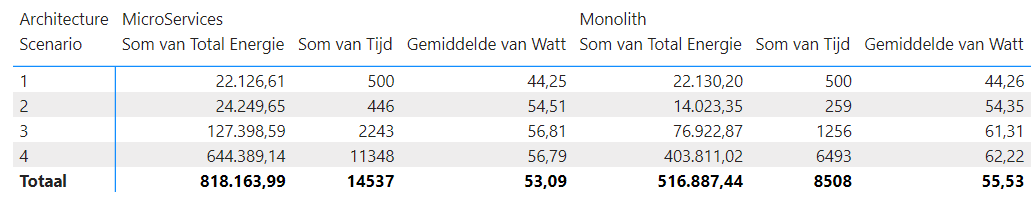
\includegraphics[scale=0.70]{apoc_totals_arch}
    \centering
    \caption{(Totale) verwerkte data per architectuur}
    \label{apoc_totals_arch}
\end{figure}

\begin{figure}[h!]
    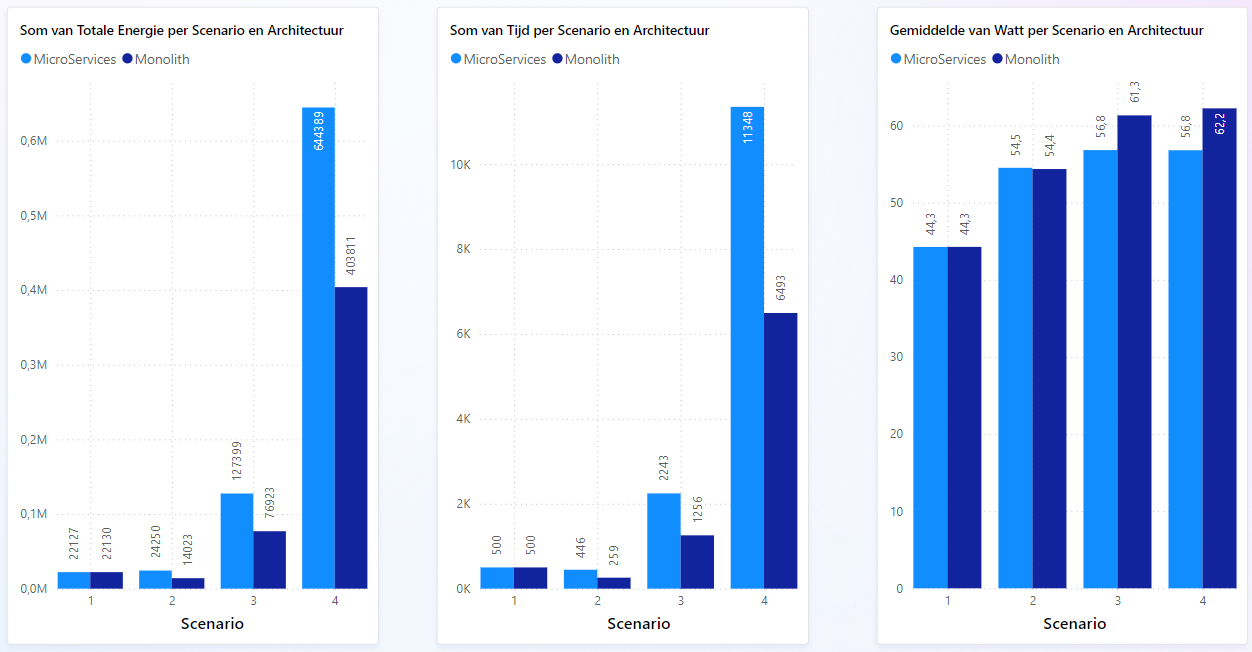
\includegraphics[scale=0.60]{apoc_3_graphs}
    \centering
    \caption{(Totale) verwerkte data in grafieken}
    \label{apoc_3_graphs}
\end{figure}


Figuur \ref{apoc_avg_watt_arch_scen} zoomt meer in op het gemiddelde watt verbruik van de applicaties. Scenario 1 en 2 lopen vrijwel gelijk. Buiten kleine fluctuaties verbruiken ze nagenoeg hetzelfde. Scenario 3 en 4 schetsen een ander beeld. Deze duiden aan dat voor elke ronde de microservice een lager gemiddeld watt verbruik heeft dan de monoliet. Ook wanneer het scenario weggelaten wordt heeft elke uitgevoerde test een lager gemiddeld watt verbruik.\\
\begin{figure}[h!]
    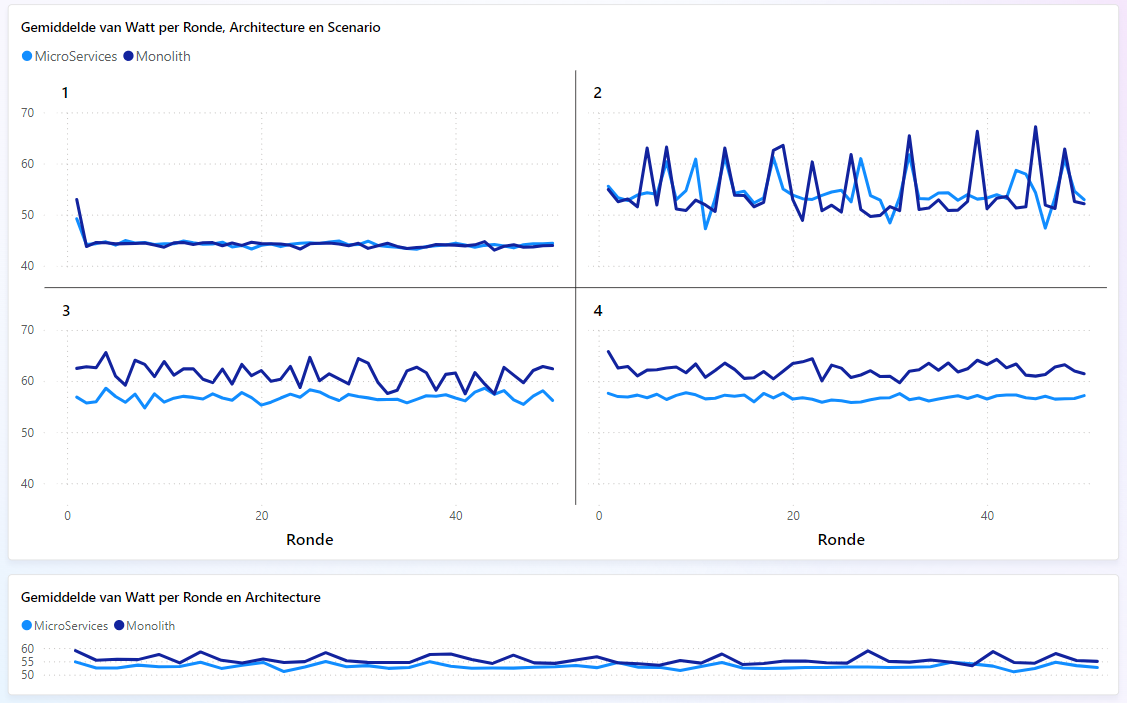
\includegraphics[scale=0.70]{apoc_avg_watt_arch_scen}
    \centering
    \caption{Gemiddelde watt verbruik per ronde, architectuur (en scenario)}
    \label{apoc_avg_watt_arch_scen}
\end{figure}


Een uitbreiding op het voorgaande is de verdeling van het gemiddelde watt verbruik per ronde, architectuur en scenario. Dit is beschikbaar in figuur \ref{apoc_avg_watt_deviation}. Uit deze grafiek blijkt dat het energieverbruik bij de microservice applicatie vaak consistenter blijft en in het algemeen lager is dan dat van de monoliet. De monoliet vertoont steeds een grotere spreiding wat wijst op meer variabiliteit en inconsistente prestaties, terwijl de microservices eerder een kleinere spreiding aanhoudt en dus consistente prestaties levert.
\begin{figure}[h!]
    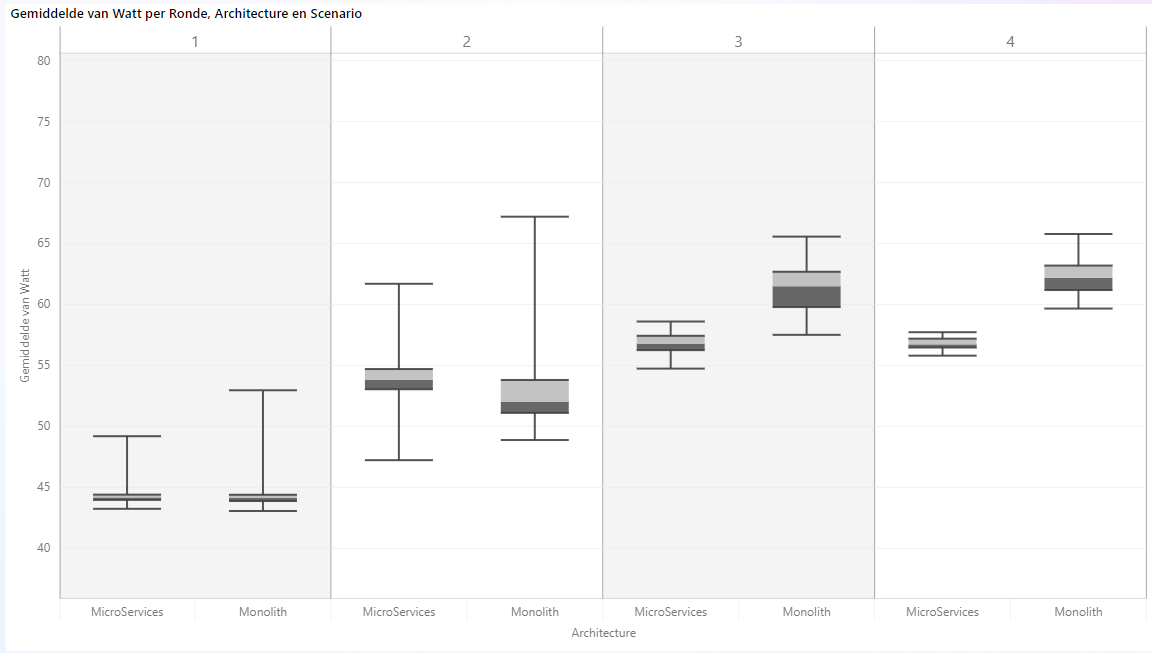
\includegraphics[scale=0.67]{apoc_avg_watt_deviation}
    \centering
    \caption{Verdeling van gemiddeld watt verbruik per ronde, architectuur en scenario}
    \label{apoc_avg_watt_deviation}
\end{figure}

\section{Interpretatie resultaten}
Wat deze resultaten vooral duidelijk maken is dat bij een idle systeem en een systeem met lage belasting, zijnde scenario 1 en 2, het verschil in energieverbruik minimaal is. Dit desondanks dat het monolithische systeem minder tijd (voor scenario 2) en energie verbruikte om deze scenario's te doorlopen. Bij een hoge belasting, hier scenario 3 en 4, verbruiken de microservices een grote hoeveelheid meer tijd en energie om de scenario's uit te voeren in vergelijking met de monoliet. Echter blijkt in alle 4 de scenario's dat het gemiddeld watt verbruik hoger is bij de monoliet en vaak ook meer onstabiel. \\

Het verschil in uitvoeringstijd kan te wijten zijn aan het feit dat de microservice applicatie via API moet wachten op een antwoord van de service waar data nodig van is. Zo wordt het voordeel van een lager gemiddeld watt verbruik opgeheven door de langere uitvoeringstijd, resulterende in een verhoogd totaal energieverbruik. Algemeen kan dus gezegd worden dat het monolithisch systeem minder energie verbruikt na het uitvoeren van totale scenario's dan de monoliet applicatie.

\section{Conclusie}
De analyse van de resultaten biedt interessante inzichten in het energieverbruik en de prestaties van microservices en monolithische applicaties onder verschillende scenario's. De belangrijkste bevindingen kunnen als volgt worden samengevat:
\begin{itemize}
    \item Microservices verbruiken \pm 3/4 meer energie dan monolithische applicaties, wat evenredig is aan de langere tijd die nodig is voor het uitvoeren van de scenario's.
    \item Ondanks het hogere totale energieverbruik, hebben microservices een lager gemiddeld wattverbruik vergeleken met monolithische applicaties.
    \item Monolithische applicaties tonen grotere spreiding en variabiliteit in hun energieverbruik, wat wijst op inconsistente prestaties.
    \item Bij lage belasting is het verschil in energieverbruik minimaal, maar bij hoge belasting  verbruiken microservices aanzienlijk meer tijd en dus ook meer energie, alhoewel ze een lager gemiddeld watt verbruik aanhouden.
\end{itemize}
